\documentclass[mathserif,xcolor=dvipsnames]{beamer}
%\usepackage{pgfpages}
%\pgfpagesuselayout{4 on 1}[letterpaper,border shrink=5mm,landscape]

\usetheme{Warsaw}
\definecolor{PittBlue}{RGB}{0.61,0.73,0.35}
\usecolortheme[named=PittBlue]{structure}
\usepackage{beamerthemesplit}
\usepackage{amsmath}
\usepackage{amsfonts}
\usepackage{xcolor}
\usepackage{multimedia}
\usepackage{caption}
\usepackage{mdwlist}
\usepackage{pgf,pgfarrows,pgfnodes}
\usepackage{helvet}
\usefonttheme{structurebold}
\usepackage{hyperref}
\setbeamertemplate{navigation symbols}{}
\setbeamertemplate{footline}{}
\definecolor{myblue}{RGB}{0,20,70}
\definecolor{mypurple}{RGB}{102,0,204}
\definecolor{mygold}{RGB}{197,179,88}
\definecolor{mygreen}{RGB}{0,128,0}
\definecolor{myorange}{RGB}{255,204,0}
\definecolor{mydarkorange}{RGB}{252,108,0}

%\setbeamercolor{title}{fg=tugred}
%\setbeamercolor{frametitle}{fg=tugred}
%\setbeamercolor{boxesroundedtitle}{fg=white,bg=myblue}
%\setbeamercolor{item projected}{fg=white,bg=myblue}

\captionsetup{labelformat=empty,labelsep=none}
\def\Tiny{\fontsize{6pt}{6pt}\selectfont}
\renewcommand{\captionfont}{\Tiny}
\def\MediumFont{\fontsize{7pt}{7pt}\selectfont}

\definecolor{tugred}{rgb}{1.0,.04,.043}

\definecolor{tugblue}{rgb}{1.0,.04,.043}
%\definecolor{tugblue}{rgb}{0.31,0.51,0.74}


\definecolor{tuggreen}{rgb}{0.61,0.73,0.35}
\definecolor{tugmagenta}{rgb}{0.50,0.39,0.64}
\definecolor{tugorange}{rgb}{0.97,0.59,0.27}

\setbeamercolor{alerted text}{fg=tugblue}
\setbeamercolor*{palette primary}{fg=gray!60!black,bg=gray!30!white}
\setbeamercolor*{palette secondary}{fg=tugred!70!black,bg=gray!15!white}
\setbeamercolor*{palette tertiary}{bg=tugred!80!black,fg=gray!10!white}
\setbeamercolor*{palette quaternary}{fg=tugred,bg=gray!5!white}

\setbeamercolor*{sidebar}{fg=tugred,bg=gray!15!white}

\setbeamercolor*{palette sidebar primary}{fg=tugred!10!black}
\setbeamercolor*{palette sidebar secondary}{fg=white}
\setbeamercolor*{palette sidebar tertiary}{fg=tugred!50!black}
\setbeamercolor*{palette sidebar quaternary}{fg=gray!10!white}

\setbeamercolor*{titlelike}{parent=palette primary}
\setbeamercolor{titlelike}{parent=pallette primary,fg=white,bg=tugred}
\setbeamercolor{frametitle}{fg=white,bg=tugred}
\setbeamercolor{frametitle right}{bg=white}

\setbeamercolor*{separation line}{}
\setbeamercolor*{fine separation line}{}

\setbeamercolor{block title}{use=structure,fg=white,bg=tugblue}
\setbeamercolor{block title alerted}{use=alerted text,fg=white,bg=alerted text.fg!75!black}
\setbeamercolor{block title example}{use=example text,fg=white,bg=example text.fg!75!black}

\setbeamercolor{block body}{parent=normal text,use=block title,bg=block title.bg!10!bg}
\setbeamercolor{block body alerted}{parent=normal text,use=block title alerted,bg=block title alerted.bg!10!bg}
\setbeamercolor{block body example}{parent=normal text,use=block title example,bg=block title example.bg!10!bg}

\setbeamercolor{itemize item}{fg=tugblue}
\setbeamercolor{itemize subitem}{fg=tugblue}
\setbeamercolor{itemize subsubitem}{fg=tugblue}

%\setbeamercolor{section/subsection in toc}{fg=tugblue}
\setbeamercolor{section in toc}{fg=black,bg=white}
\setbeamercolor{subsection in toc}{fg=black,bg=white}

\setbeamercolor{structure}{fg=tugblue}

\setbeamertemplate{itemize subitem}{\rule{4px}{4px}}

%\mode<presentation>
{
%  \useoutertheme{default}   % empty
%  \useoutertheme{infolines}% simple but bland
 % \useoutertheme{split}    % ok if compress option used
%  \useoutertheme{shadow}   % way too much space used -- ok with option 'compress'
  %\useoutertheme{shadow}   
  %\setbeamercovered{transparent} % or whatever (possibly just delete it)
  %\useoutertheme[subsection=false]{miniframes}
}

\makeatletter
\setbeamertemplate{footline}
{
  \leavevmode%
  \hbox{%
  \begin{beamercolorbox}[wd=.3333\paperwidth,ht=2.25ex,dp=1ex,center]{author in head/foot}%
    \usebeamerfont{author in head/foot}%\insertshortauthor
    ~~\beamer@ifempty{\insertshortinstitute}{}{\insertshortinstitute}
  \end{beamercolorbox}%
  \begin{beamercolorbox}[wd=.3333\paperwidth,ht=2.25ex,dp=1ex,center]{title in head/foot}%
    \usebeamerfont{title in head/foot}\insertshorttitle
  \end{beamercolorbox}%
  \begin{beamercolorbox}[wd=.3333\paperwidth,ht=2.25ex,dp=1ex,right]{date in head/foot}%
%    \usebeamerfont{date in head/foot}\insertshortdate{}\hspace*{2em}
    \insertframenumber{} / \inserttotalframenumber\hspace*{2ex} 
  \end{beamercolorbox}}%
  \vskip0pt%
}
\makeatother



\makeatletter
\def\blfootnote{\xdef\@thefnmark{}\@footnotetext}
\makeatother


\setbeamertemplate{caption}{\raggedright\insertcaption\par}\newtheorem{conjecture}{Conjecture}[section]
\newtheorem{conj}{Conjecture}[section]

\newtheorem{cor}{Corollary}[section]
\newtheorem{question}{Question}[section]

\newtheorem{answer}{Answer}[section]
\newtheorem{idea}{Idea}[section]

\newtheorem{exercise}{Exercise}[section]
\newtheorem{riddle}{Riddle}[section]


\newtheorem{remark}{Remark}[section]
\newtheorem{proposition}{Proposition}[section]
\newtheorem{assumption}{Assumption}[section]
\newtheorem{conditions}{Conditions}[section]
\newtheorem{tfram}{\hspace{0cm}}[section]

\usepackage{xcolor,soul}
\definecolor{lightblue}{rgb}{.90,.95,1}
\sethlcolor{lightblue}
\renewcommand<>{\hl}[1]{\only#2{\beameroriginal{\hl}}{#1}}

% http://tex.stackexchange.com/questions/41683/why-is-it-that-coloring-in-soul-in-beamer-is-not-visible
\makeatletter
\newcommand\SoulColor{%
  \let\set@color\beamerorig@set@color
  \let\reset@color\beamerorig@reset@color}
\makeatother
\SoulColor


\newcommand{\con}{\operatorname{Conf}}
\newcommand{\bcon}{\operatorname{BConf}}
\newcommand{\DOD}{\operatorname{DOD}}
\newcommand{\FCC}{\operatorname{FCC}}
\newcommand{\HCP}{\operatorname{HCP}}
\newcommand{\RR}{{\mathbb R}}
\def\SS{\mathbb{S}}
\newcommand{\bU}{{\bf U}}

\newcommand{\bV}{{\bf V}}
\newcommand{\bu}{{\bf u}}
\newcommand{\bv}{{\bf v}}
\newcommand{\sL}{{\mathcal L}}


\usepackage{diagbox}
\usepackage{media9}
\usepackage{tikz}






\title[Critical Packings]{Critical packings, rigidity, and the radius function}
\author{W\"oden Kusner}
\institute[Math A]{Institute for Analysis and Number Theory  \\ Graz University of Technology \\[.5em]

\includegraphics[height=0.5in]{logo.pdf}}
\date{\small{January  2017}}



\begin{document}




%%%%%%%%%%%%%%%%%%%%%%%%%%
%
%   
%
%%%%%%%%%%%%%%%%%%%%%%%%%%




\frame[plain]{\vspace{.25in}\titlepage}



%%%%%%%%%%%%%%%%%%%%%%%%%%
%
%   
%
%%%%%%%%%%%%%%%%%%%%%%%%%%


\frame{
\frametitle{\hspace{0cm}}
\begin{abstract}
\tiny
There are a number of classical problems in geometric optimization that ask for the "best" configuration of points with respect to some function. We are interested in the relationships between various notions of criticality for such functions on configuration spaces, in particular the injectivity or packing radius.  This is not a Morse function, but it has been observed to be Morse-like, in that the topological notion of regularity can be defined in an analogous way.  Furthermore, there is a geometric interpretation from rigidity theory that characterizes configurations as critical by the existence of a strut measure.  

\end{abstract}
\vspace{2em}
\centering
\tiny
Based on work with\\ Robert Kusner, Jeffrey Lagarias \& Senya Shlosman\\ arXiv 1611.10297
}


%%%%%%%%%%%%%%%%%%%%%%%%%%
%
%  
%
%%%%%%%%%%%%%%%%%%%%%%%%%%

\frame{
\frametitle{Tammes Problem: P. M. L. Tammes (1930)}
\begin{columns}[t]
\begin{column}{.6\textwidth}
\vspace{-.5cm}
\begin{question}What is the maximal radius possible for $\,N$ equal spheres, all touching a central sphere of radius $\,1$?\end{question}

The original formulation of the \emph{Tammes problem}: How many spherical caps of angular diameter $\theta$ that can be placed without overlap? \newline\newline
\onslide<2,3>{
Tammes was studying pollen grains and empirically determined $6$ for $\theta = \frac{2\pi}{4}$ but no more than $4$ for $\theta > \frac{2\pi}{4}$.  }
\end{column}
\begin{column}{.3\textwidth}
\centering
\vspace{-1cm}
\begin{figure}[htbp] %  figure placement: here, top, bottom, or page
   \centering
   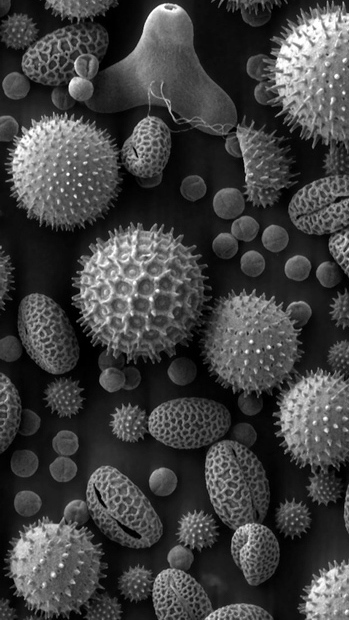
\includegraphics[width=1.3in]{imagesattalk/pollen} 
   \end{figure}
\end{column}
\end{columns}
\onslide<3>{\begin{remark}
\centering The maximizing configuration for $5$ is not unique.\end{remark}}
}

%%%%%%%%%%%%%%%%%%%%%%%%%%
%
%  
%
%%%%%%%%%%%%%%%%%%%%%%%%%%

\frame{
\frametitle{Tammes Problem: L. Fejes-T\'{o}th (1943)}

The Tammes problem was initially solved for $N= 3, 4, 6$ and $12$, with configurations of cap centers for $N=3$ attained by vertices of an equatorial equilateral triangle and for $N=\{4, 6, 12\}$ by vertices of regular tetrahedron, octahedron and icosahedron. 

\begin{figure}[htbp] %  figure placement: here, top, bottom, or page
   \centering
      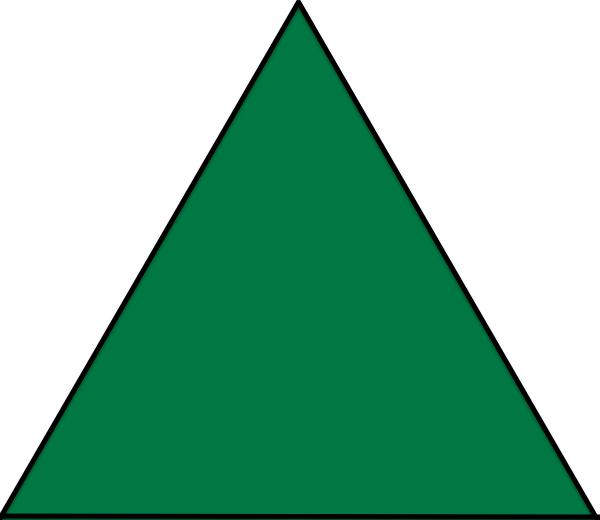
\includegraphics[width=1in]{imagesattalk/tri1.png} 
   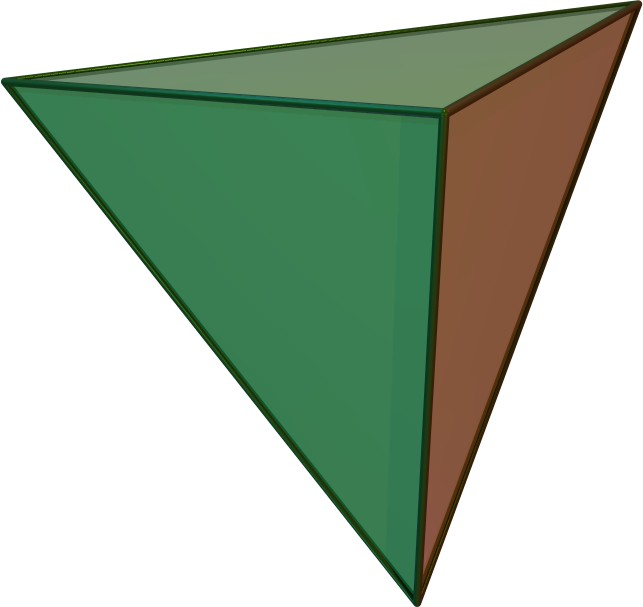
\includegraphics[width=1in]{imagesattalk/tet1.jpg} 
    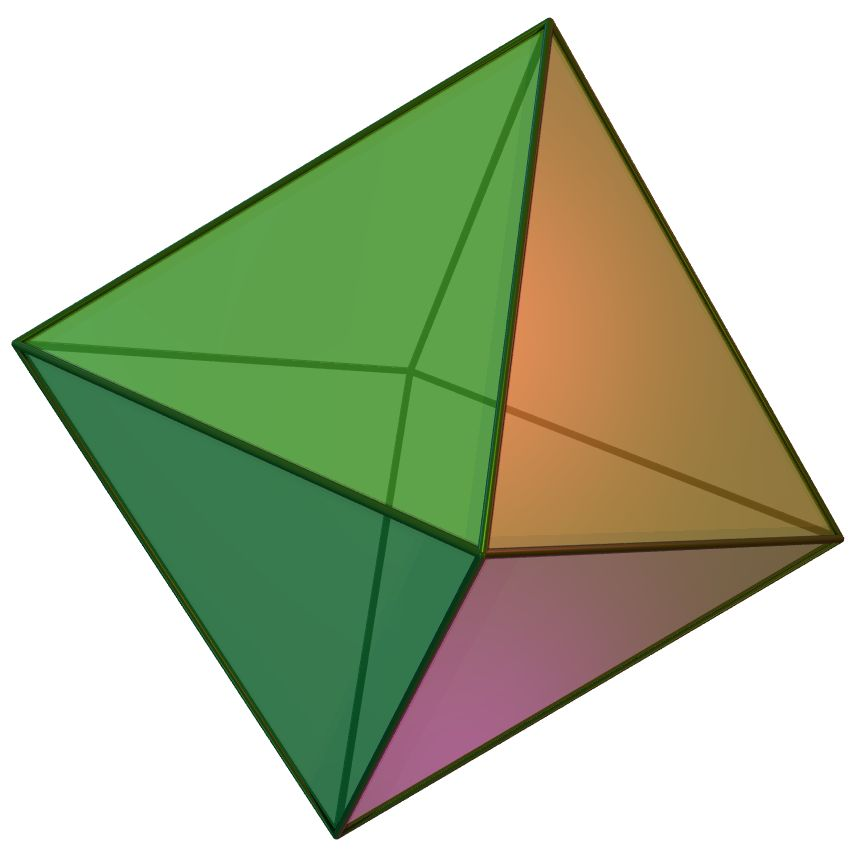
\includegraphics[width=1in]{imagesattalk/oct1.jpg} 
     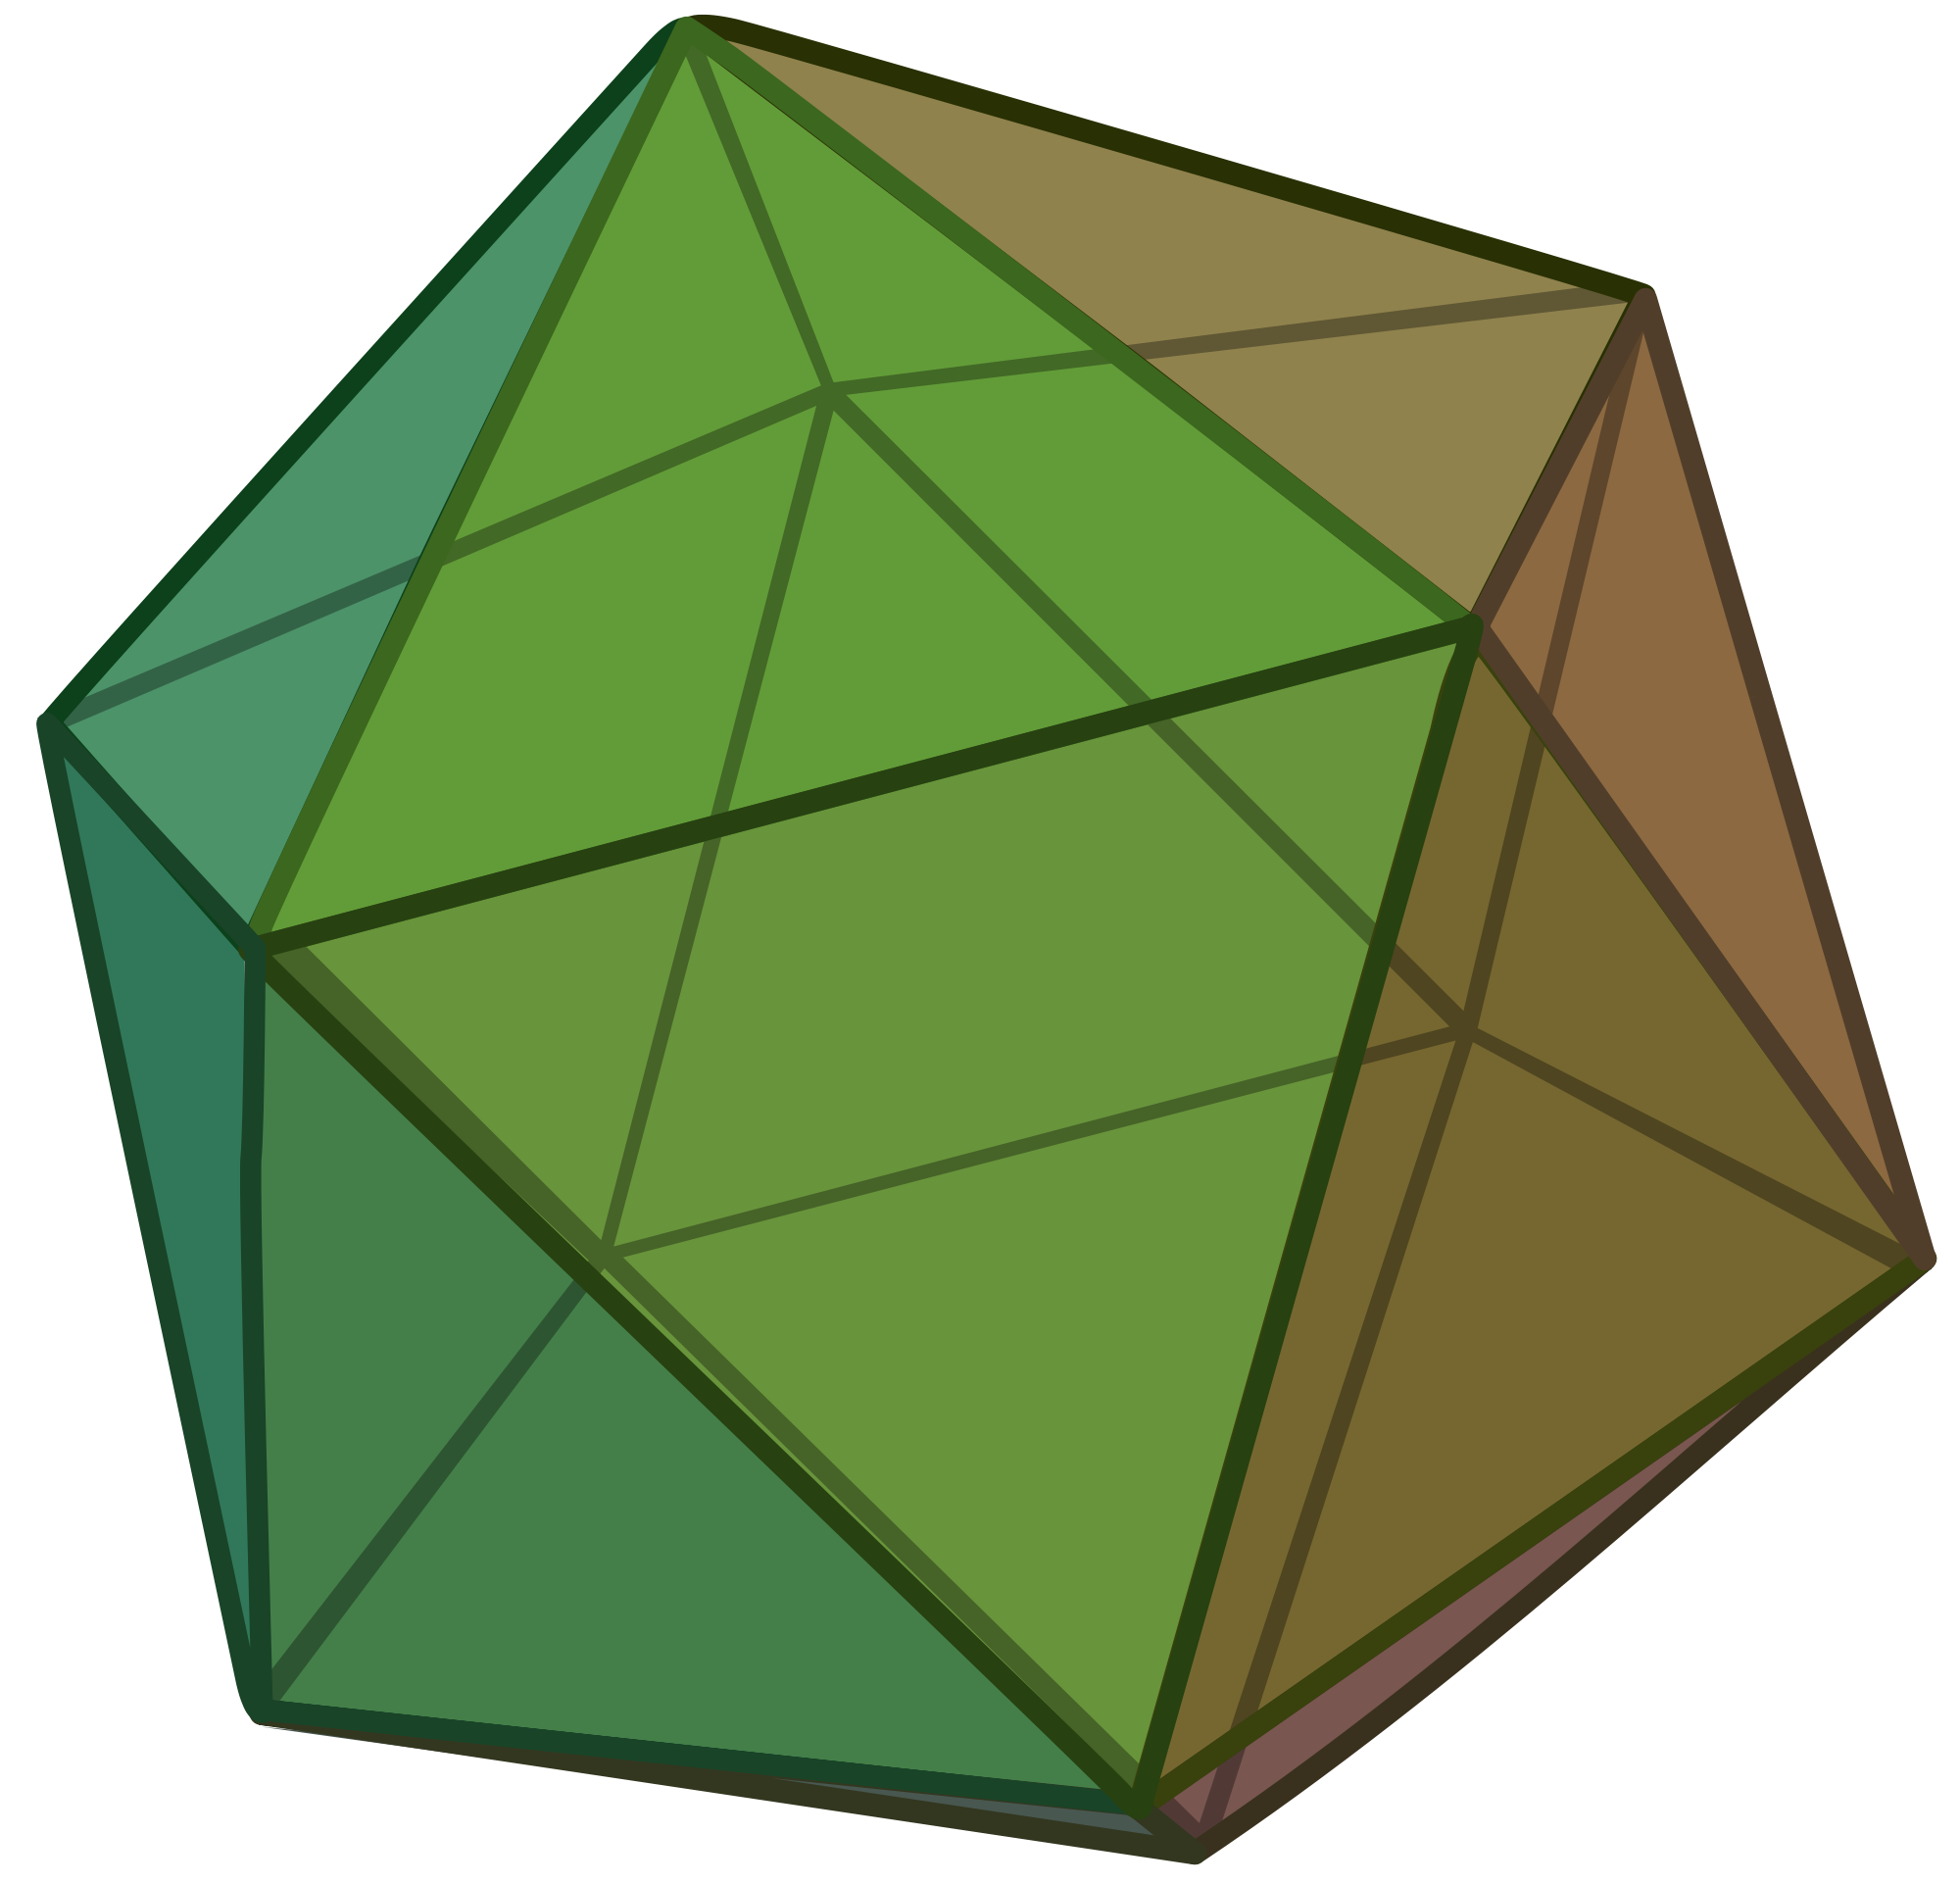
\includegraphics[width=1in]{imagesattalk/ico1.png} 
\end{figure}
}


%%%%%%%%%%%%%%%%%%%%%%%%%%
%
%   
%
%%%%%%%%%%%%%%%%%%%%%%%%%%

\frame{
\frametitle{Tammes Problem: Other $N$}
\begin{columns}[t]
\begin{column}{.50\textwidth}
The Tammes problem has been solved exactly for only $3 \le N \le 14$ and $N=24$. It was solved for $N=\{5, 7, 8, 9\}$ by Sch\"{u}tte and van der Waerden in 1951, $N=\{10, 11\}$ by Danzer in his 1963 Habilitationsschrift. 
\vspace{.5cm}
\begin{figure}[htbp] %  figure placement: here, top, bottom, or page
   \centering
     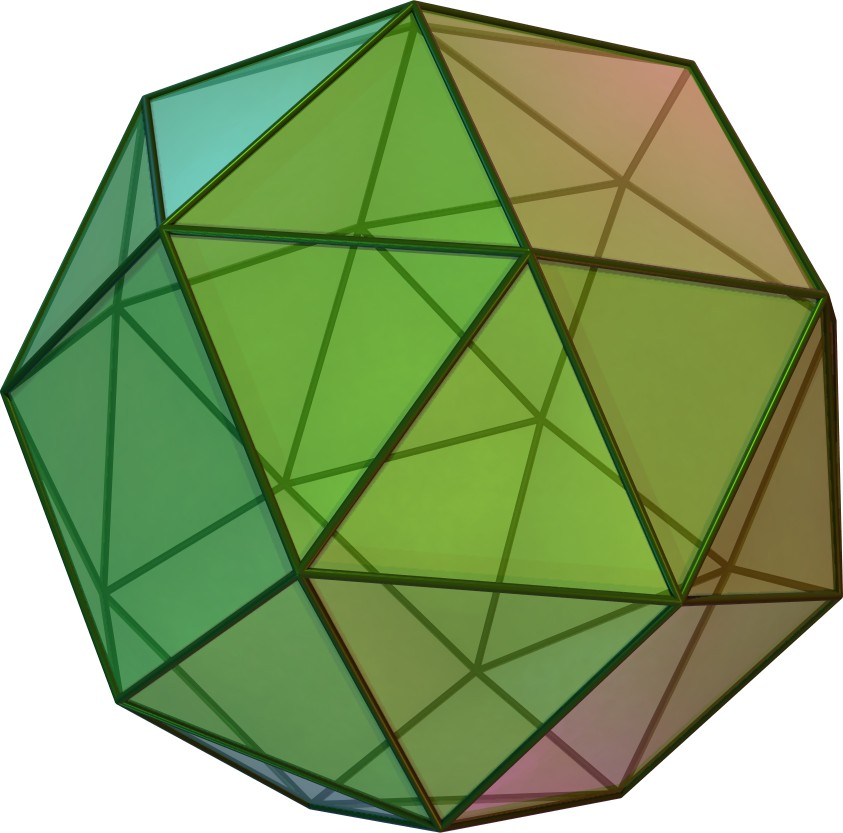
\includegraphics[width=1in]{imagesattalk/snub1.jpg} 
\end{figure}

\end{column}
\begin{column}{.5\textwidth}
\vspace{-.5cm}
\begin{figure}[htbp] %  figure placement: here, top, bottom, or page
   \centering
   \hspace{-2em}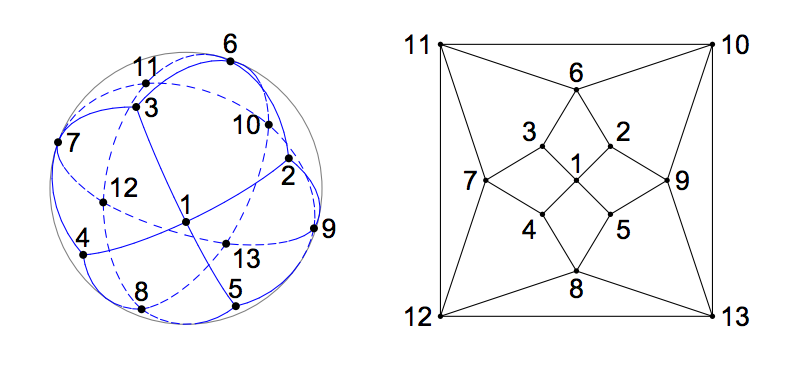
\includegraphics[width=2in]{imagesattalk/musin.png} 
\end{figure}\vspace{-1em}
The case $N=24$ was solved by Robinson in 1961 showing the configuration of centers were the vertices of a snub cube.  The cases $N=\{13, 14\}$ were solved by Musin and Tarasov, enumerating all plausible graphs by computer. 
\end{column}
\end{columns}
}


%%%%%%%%%%%%%%%%%%%%%%%%%%
%
%   
%
%%%%%%%%%%%%%%%%%%%%%%%%%%

\frame{
\frametitle{Critical Packings}
\begin{question}
We have some solutions for the global maxima for the Tammes Problem, but there could be other interesting configurations.
What about other critical points?  Are there local \emph{maxima}?
\end{question}

\onslide<2>{

\begin{figure}[htbp] %  figure placement: here, top, bottom, or page
   \centering
         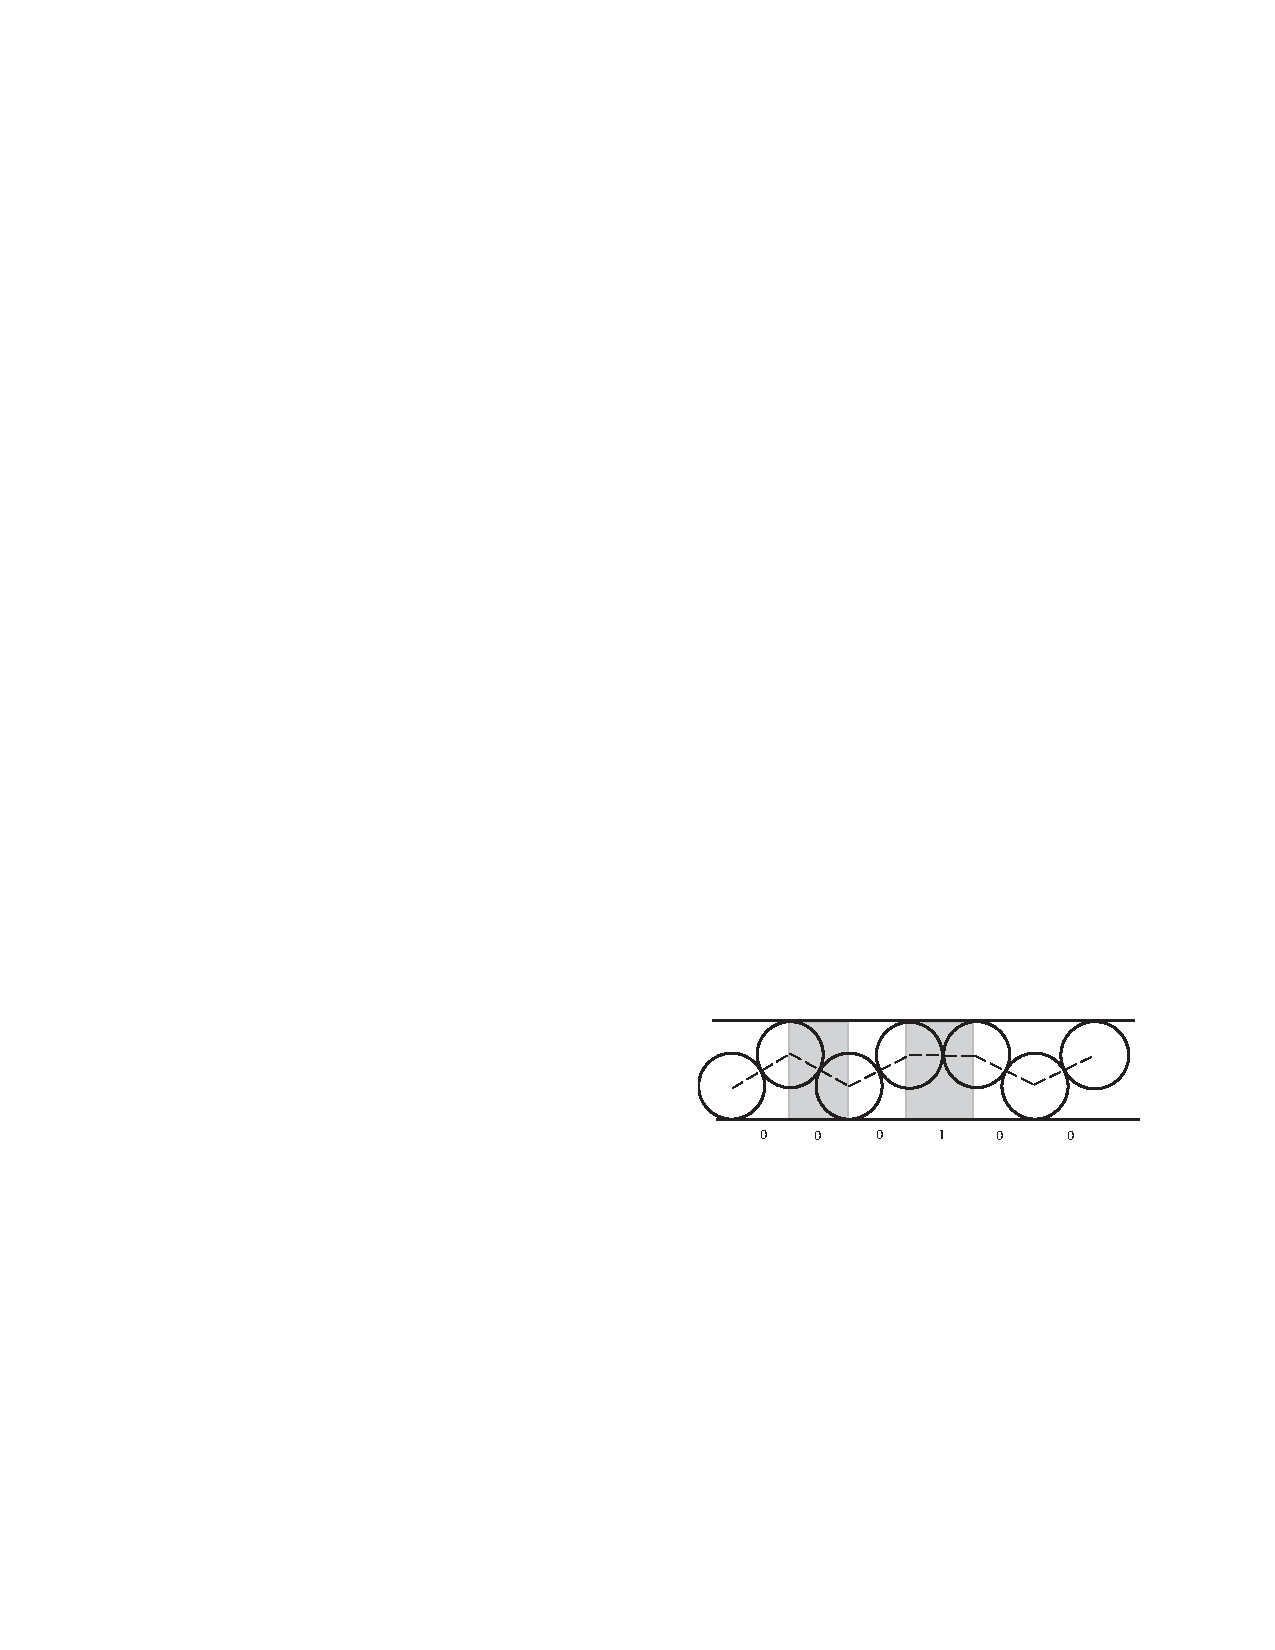
\includegraphics[width=3in]{imagesattalk/q1d} 
  \end{figure}

\begin{remark}
One ``similar'' model that can be analyzed completely is the quasi-1D packing problem.  Such packings have lots of maxima.
\end{remark}
}
}





%%%%%%%%%%%%%%%%%%%%%%%%%%
%
%   
%
%%%%%%%%%%%%%%%%%%%%%%%%%%


\frame{
\frametitle{Key Players}


\begin{definition}
The classical {\em configuration space} $\con(N) := \con(\SS^2,N)$ of $N$ distinct labeled points on the unit $2$-sphere $\SS^2$.
\end{definition}
\begin{definition}
The {\em reduced configuration space}
\[
\bcon(N) := \con(N) / SO(3).
\]
Assume $N \ge 3$ to avoid degenerate cases. \end{definition}

\begin{definition}
 Configurations are $\bU:= (\bu_1, \bu_2, ..., \bu_N)$, where the  $\bu_j \in \SS^2$ are distinct points.
\end{definition}

}



%%%%%%%%%%%%%%%%%%%%%%%%%%
%
%   
%
%%%%%%%%%%%%%%%%%%%%%%%%%%

\frame{
\frametitle{Key Players}

\begin{definition}
The {\em injectivity radius function} $\rho: \, \con(N) \to \RR^{+}$ assigns  a
configuration $\bU:= (\bu_1, \bu_2, \dots, \bu_N) \in (\SS^2)^N$ the value
\[
\rho(\bU) := \frac{1}{2} \big( \min_{i \ne j} \theta(\bu_i, \bu_j) \big),
\]
where $\theta(\bu_i, \bu_j)$ is the angular distance between $\bu_i$ 
and $\bu_j$.  
\end{definition}

\begin{remark}
Since $\rho$ is invariant under the action of $SO(3)$,
it decends to a well-defined function on $\bcon(N; \theta)$, which we also denote $\rho$. 
\end{remark}
\begin{definition}
\[
\con(N; \theta) :=  \{ \bU= (\bu_1, ..., \bu_N) :  \, \rho(\bU) \ge \frac{\theta}{2} \}.
\]
\end{definition}

}




%%%%%%%%%%%%%%%%%%%%%%%%%%
%
%   
%
%%%%%%%%%%%%%%%%%%%%%%%%%%


\frame{
\frametitle{Morse Theory}

\emph{Morse theory} concerns how topology changes for the super level
sets of a smooth real-valued function on a manifold.  
\begin{definition}[super level set]
For $f: M \rightarrow \RR$, $M^a := \{x\in M : f(x) \ge a \}$ is a superlevel set.
\end{definition}

\begin{theorem}
Given a smooth function $f: M \rightarrow \RR$ and an interval $[a,b]$ with compact preimage, and $[a,b]$ contains no critical values.  Then $M^a$ is diffeomorphic to $M^b$.  
\end{theorem}

It is at the \emph{critical values} of the function that the topology of the super level changes.
}




%%%%%%%%%%%%%%%%%%%%%%%%%%
%
%   
%
%%%%%%%%%%%%%%%%%%%%%%%%%%

\frame{
\frametitle{Morse Theory}

To vary a configuration $\bU=(\bu_1,...,\bu_N) \in \con(N)\subset (\SS^2)^N$ along a tangent vector $\bV=(\bv_1,...,\bv_N)$ to $\con(N)$ at $\bU$, 
 use an ersatz exponential map.

For sufficiently small $\bV$, define a nearby configuration 
$$\bU\#\bV=(\frac{\bu_1+\bv_1}{| \bu_1+\bv_1|},..., \frac{\bu_N+\bv_N}{| \bu_N+\bv_N|}) \in \con(N)\subset (\SS^2)^N$$ 
by summing and projecting each factor back to $\SS^2$.  

In particular, the $\bV$-directional derivative of a smooth function $f$ on $\con(N)$ at $\bU$ is $\frac{d}{dt}|_{t=0} f(\bU\#t\bV)$.

\onslide<2>{
\begin{definition}
 $\bU$ is a critical point for smooth $f$ provided all its $\bV$-derivatives vanish at $\bU$. That is, the increment
$f(\bU\#\bV)-f(\bU) = o(\bV).$
\end{definition}}
}



%%%%%%%%%%%%%%%%%%%%%%%%%%
%
%   
%
%%%%%%%%%%%%%%%%%%%%%%%%%%

\frame{

\frametitle{Morse Theory}

\begin{remark}
\centering
The injectivity radius function is not Morse.
\end{remark}


The injectivity radius function $\rho$ on $\con(N)$ is not smooth: it is a min-function for a finite number of smooth functions. 
But we may still be inspired by Morse theory to pass between the topological, analytic and geometric notions of ``critical''.


\onslide<2>{
\begin{definition}
A  configuration  $\bU=(\bu_1,...,\bu_N) \in \con(N)$ is {\em critical for maximizing} $\rho$ provided for every sufficiently
small $\bV=(\bv_1,...,\bv_N)$,  we have $\max[\rho(\bU\#\bV)-\rho(\bU),0] = o(\bV)$.  
That is, a configuration $\bU$ is \emph{critical for maximizing} if there is no variation $\bV$ that can increase $\rho$ to first order.  
\end{definition}
}


}




%%%%%%%%%%%%%%%%%%%%%%%%%%
%
%   
%
%%%%%%%%%%%%%%%%%%%%%%%%%%


\frame{
\frametitle{Morse Theory}


If we are not critical for maximizing, there exists a variation $\bV$ which increases $\rho$ to first order.  By the definition of $\rho$ as a min-function, the distance between all pairs $(\bu_i, \bu_j)$ realizing the minimal angular distance $\theta(\bu_i, \bu_j)= \theta_o$ increases to first order along $\bV$.  So there is also a notion of regular value analogous to the smooth case.


\onslide<2>{
\begin{theorem}[Topological Regularity]
If such a variation exists for all configurations in this $\rho=\theta_o$-level set, then this level is {\em topologically regular:} 
that is, the variations provide a deformation retraction from $\con(N;\theta_o-\varepsilon)$ to $\con(N;\theta_o+\varepsilon)$ for some $\varepsilon>0$.
\end{theorem}
}

}



%%%%%%%%%%%%%%%%%%%%%%%%%%
%
%   
%
%%%%%%%%%%%%%%%%%%%%%%%%%%

\frame{
\frametitle{Balanced Graphs}


\begin{columns}[t]
\begin{column}{.7\textwidth}

\begin{definition}\label{def:47}
For $\bU \in \con(N; \theta)$, the  {\em contact graph} of $\bU$ is the graph embedded in $\SS^2$ with vertices given by points 
$\bu_i$ in $\bU$ and edges given by the geodesic segments $[\bu_i, \bu_j]$ when $d(\bu_i , \bu_j) =\theta$.  
\end{definition}

\begin{definition}\label{def:48}
 A {\em stress graph} for $\bU \in \con(N; \theta)$ is a contact graph with nonnegative weights $w_e$ on each geodesic edge $e=[\bu_i, \bu_j]$.
\end{definition}




\end{column}
\begin{column}{.3\textwidth}
\centering

\begin{figure}[htbp] %  figure placement: here, top, bottom, or page
   \centering
   \vspace{.5in}
         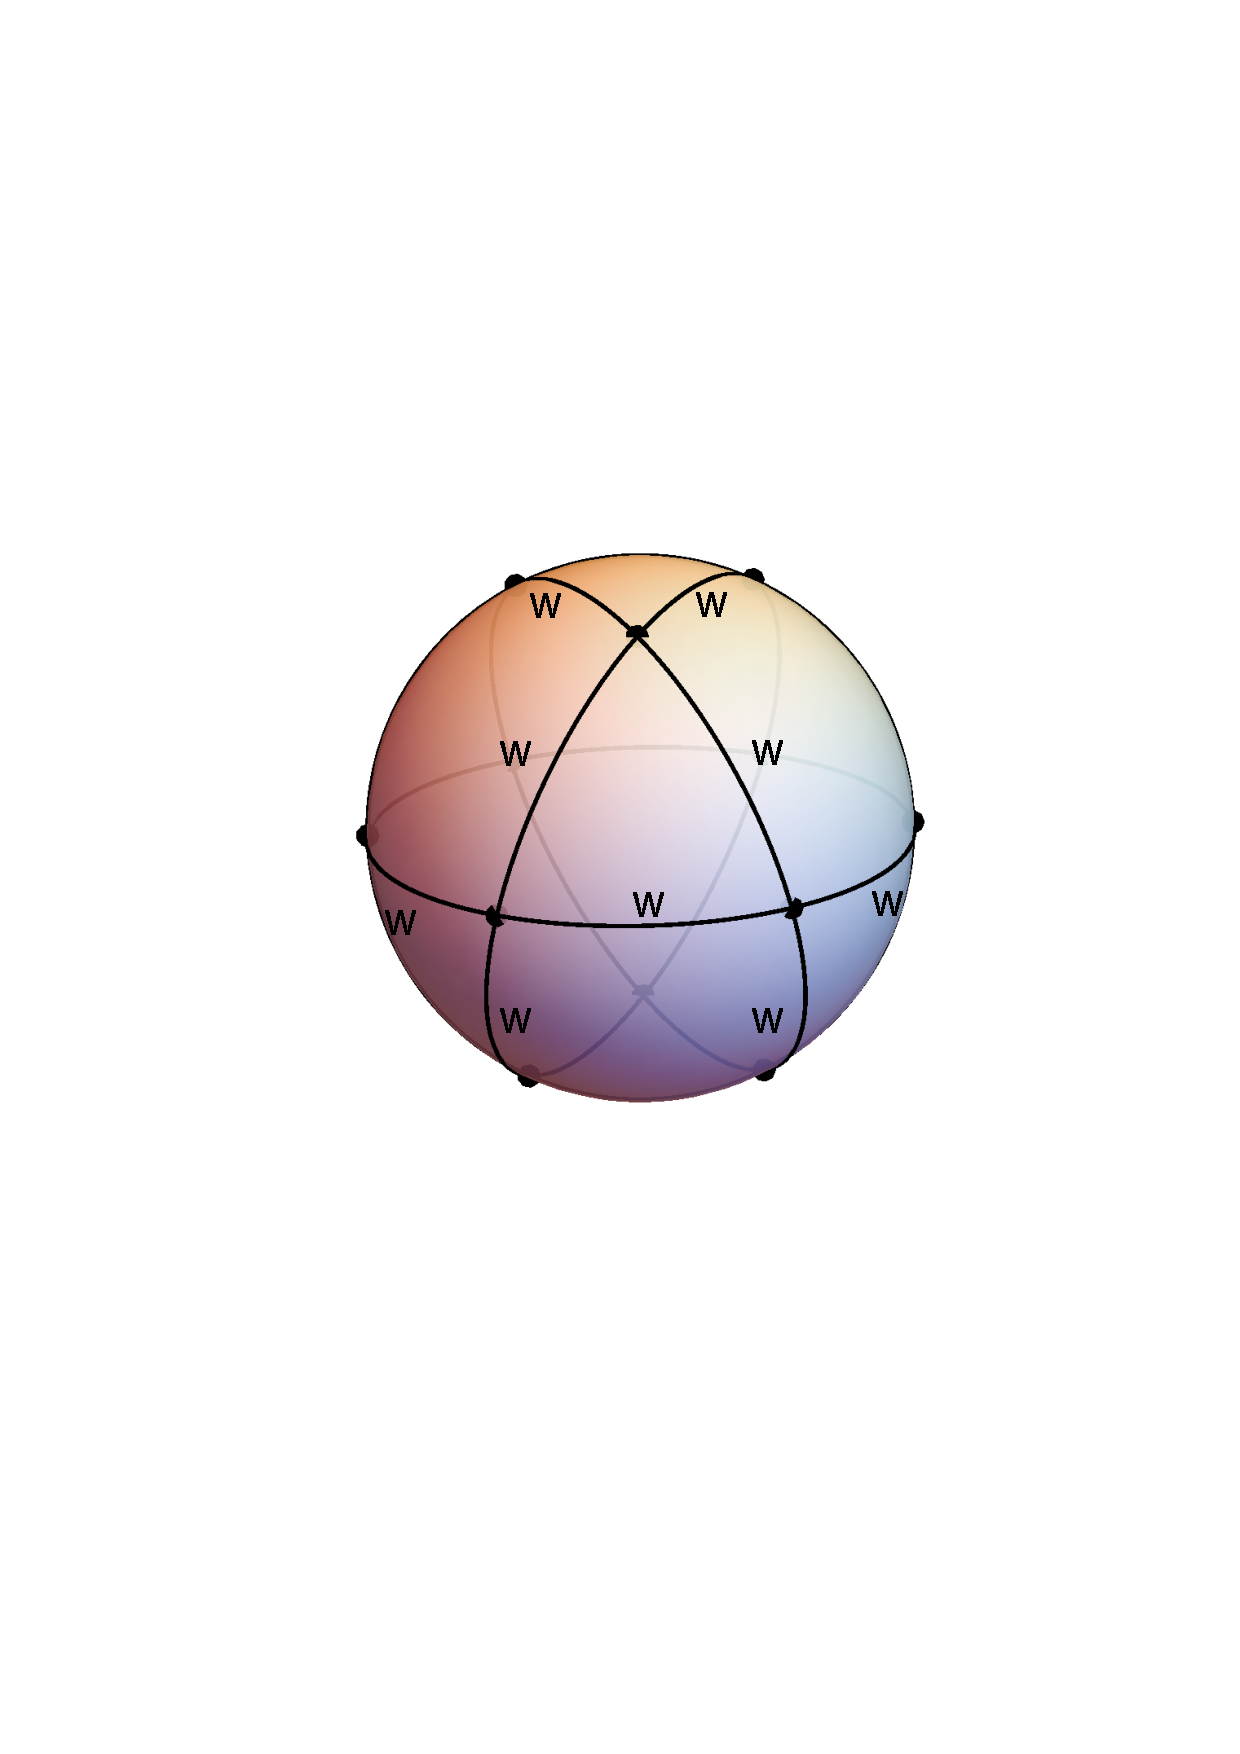
\includegraphics[width=1.2in]{imagesattalk/FCCstressgraph(cropped)}

                  \label{fig:contact}
\end{figure}

\end{column}
\end{columns}

}



%%%%%%%%%%%%%%%%%%%%%%%%%%
%
%   
%
%%%%%%%%%%%%%%%%%%%%%%%%%%


\frame{
\frametitle{Balanced Graphs}

\begin{columns}[t]
\begin{column}{.7\textwidth}

A stress graph associates a system of {\em tangential forces} to edges $e=[\bu_i, \bu_j]$ of the contact graph. The forces have magnitude $w_e$, are tangent to $\SS^2$ at each point $\bu_i$ of $\bU$, and point outward at the ends of each edge. 


\begin{definition} A stress graph is  {\em balanced} if the sum of the forces
in $T_{\bu_i}\SS^2$ is zero for all points of $\bU.$  A configuration $\bU$ is {\em balanced} if it has a balanced stress graph for some choice of non-negative, not everywhere zero weights on its edges.
\end{definition}



\end{column}
\begin{column}{.3\textwidth}
\centering

\begin{figure}[htbp] %  figure placement: here, top, bottom, or page
   \centering
 \vspace{.5in}
     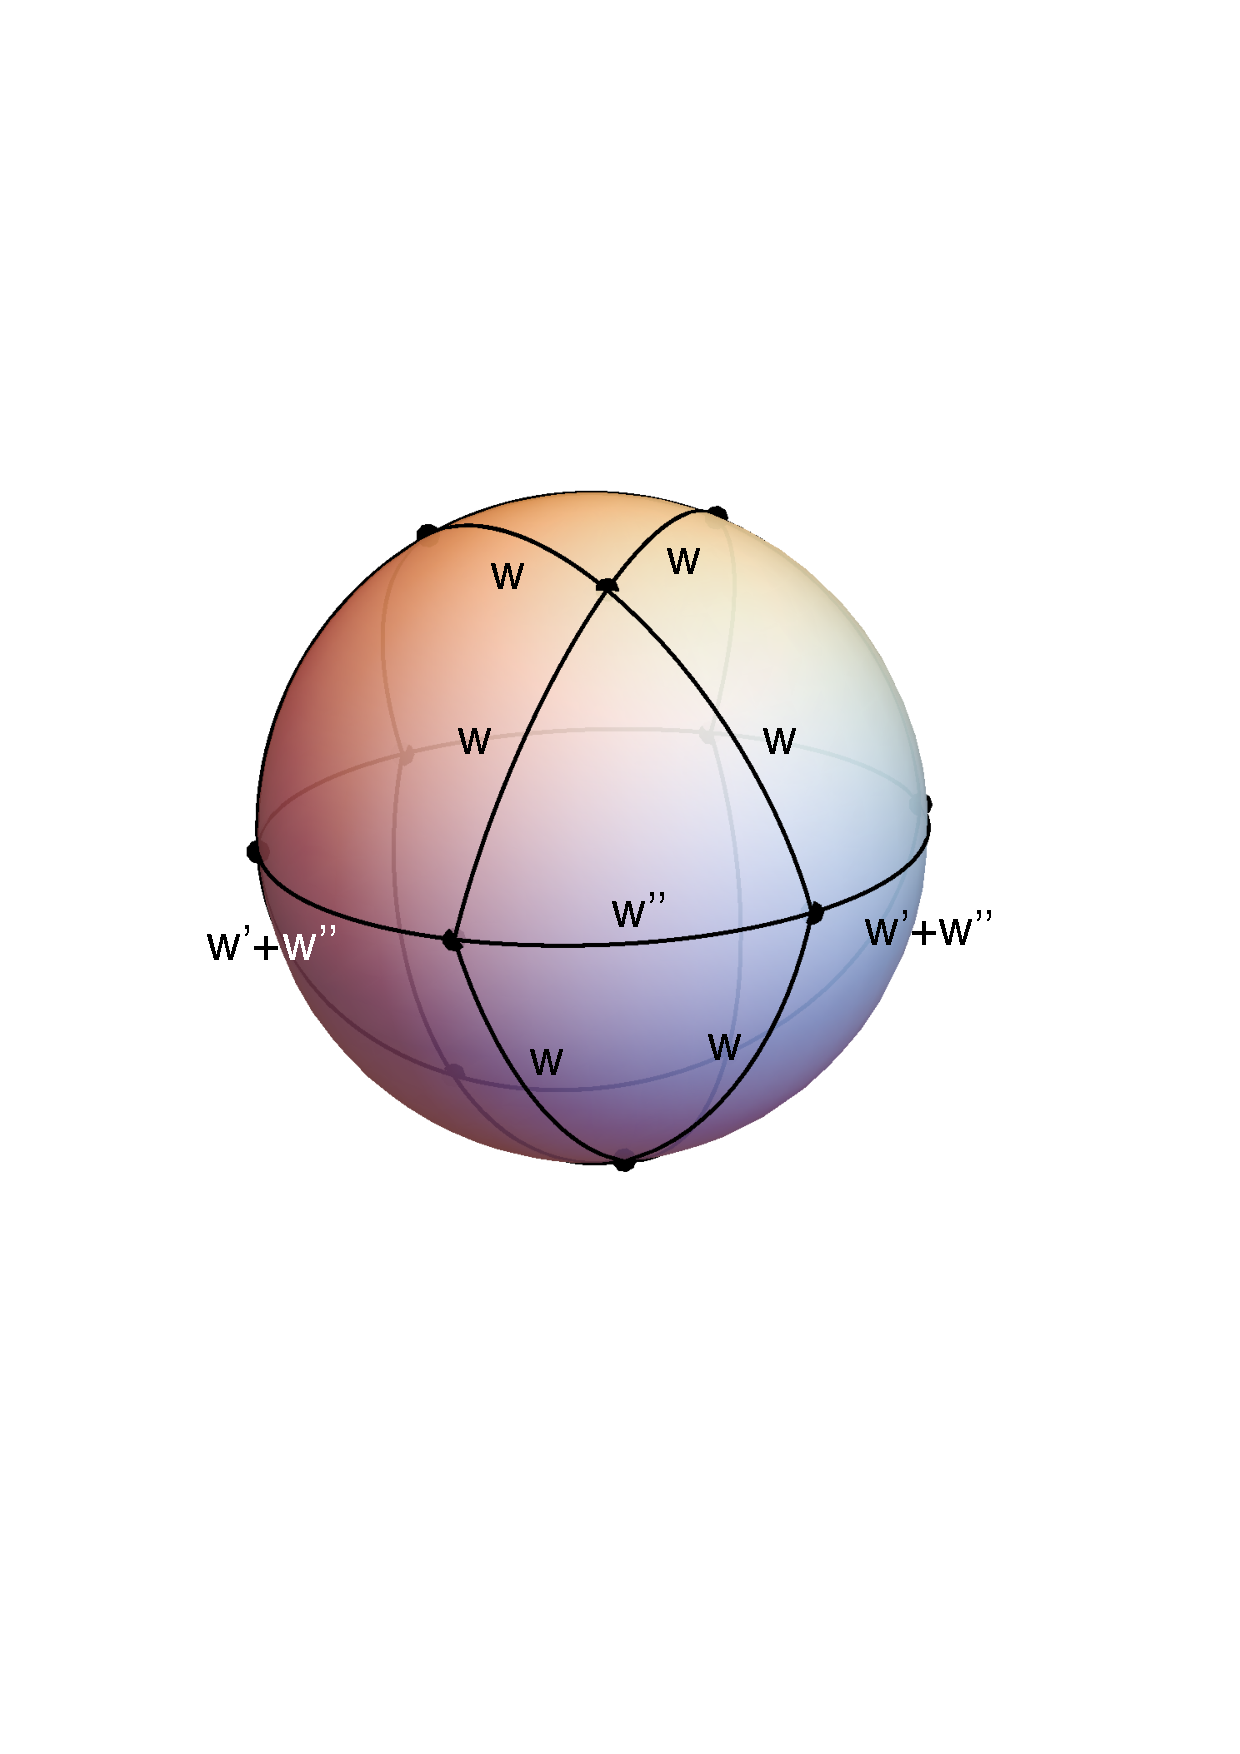
\includegraphics[width=1.23in]{imagesattalk/HCPstressgraph(cropped)} 

                  \label{fig:contact}
\end{figure}

\end{column}
\end{columns}

}



%%%%%%%%%%%%%%%%%%%%%%%%%%
%
%   
%
%%%%%%%%%%%%%%%%%%%%%%%%%%


\frame{
\frametitle{Balanced Graphs}


\begin{theorem} \label{thm:contact}
For each topologically critical value $\theta$ for  the injectivity radius $\rho$, there exists a balanced configuration $\bU$. The vertices of the contact graph are a subset of the points in $\bU$ and the geodesic edges of the contact graph all have length $\theta$.
\end{theorem}


\begin{theorem} \label{thm:converse}
 If a configuration ${\bf U}$ on $\SS^2$ is balanced, then ${\bf U}$ is critical for maximizing the injectivity radius $\rho$.
\end{theorem}

}



%%%%%%%%%%%%%%%%%%%%%%%%%%
%
%   
%
%%%%%%%%%%%%%%%%%%%%%%%%%%


\frame{
\frametitle{Summary}


\begin{columns}[t]\vspace{-2em}
\begin{column}{.60\textwidth}
There are certain radii that are critical:  The topology of the configuration space changes.  
\newline

These radii also correspond to configurations of points that are force balanced:  There exists a non-trivial strut measure on the contact graph that force balances all the vertices.
\newline

Such configurations obstruct the $\rho$-subgradient flow, which would give a deformation retraction.


\end{column}

\begin{column}{.40\textwidth}

\begin{figure}[htbp] %  figure placement: here, top, bottom, or page
   \centering
   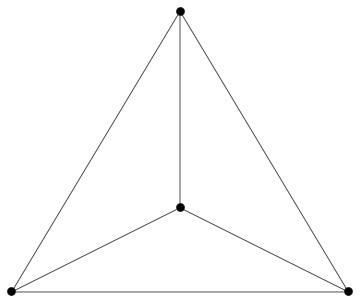
\includegraphics[width=1in]{imagesattalk/n4.jpg} 

\end{figure}

\begin{figure}[htbp] %  figure placement: here, top, bottom, or page
   \centering
   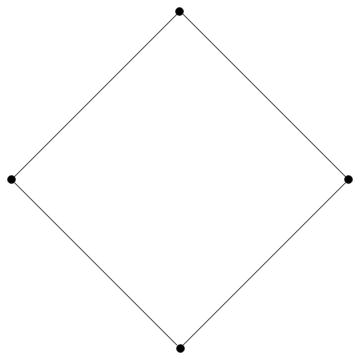
\includegraphics[width=1in]{imagesattalk/graph4.jpg} 

\end{figure}

\end{column}
\end{columns}



}



%%%%%%%%%%%%%%%%%%%%%%%%%%%
%%
%%   
%%
%%%%%%%%%%%%%%%%%%%%%%%%%%%


\frame{
\frametitle{Exploring Configuration Space}

\begin{remark}
The configuration space of points on the sphere is a nice space to experiment with.  
It inherits a nice metric, the tangent space is easy to work with, it is trivial to sample, the symmetries are natural.
\end{remark}
\onslide<2>{

We can hack together a sub-gradient descent algorithm for the injectivity radius function. With that, it is a quick step to make some conjectures about local maxima, global maxima, and the distribution of maxima just by exploring the basins of attraction randomly.

}

\onslide<2>{
\vspace{-1em}
\begin{figure}[htbp] %  figure placement: here, top, bottom, or page
   \centering
 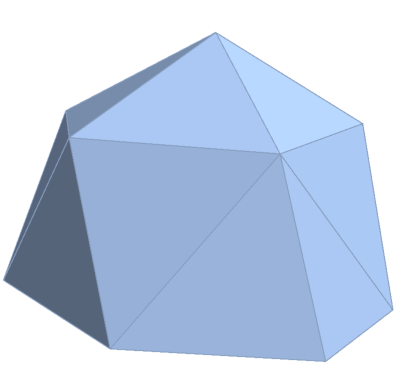
\includegraphics[width=1in]{imagesattalk/12local} 
  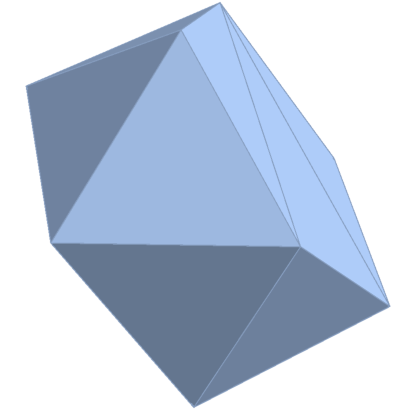
\includegraphics[width=1in]{imagesattalk/10local} 
   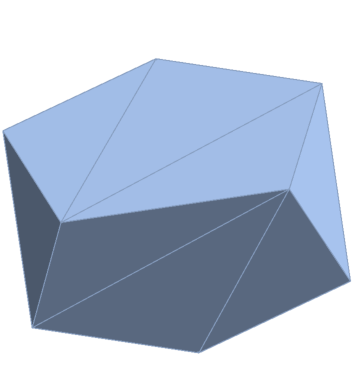
\includegraphics[width=1in]{imagesattalk/10local2} 
\end{figure}

}






}






\frame{
\frametitle{Thank you for your attention!}

\centering
wkusner.github.io
  
Supported by Austrian Science Fund (FWF) Project 5503 

}



\end{document}

